% -----------------------------------------
\chapter{Resultados e discussões}\label{chp:LABEL_CHP_5}
\label{resultados}
% -----------------------------------------
Com a utilização de \textit{frameworks} modernos, foi possível criar uma aplicação web responsiva e fluida. Ao se comparar com o estado inicial, os mockups seguiram seus propósitos e com base neles, foi possível a criação de todas as telas do sistema, conforme visto no capítulo \ref{chp:LABEL_CHP_5}. A figura \ref{home} demonstra a tela inicial, que todas as pessoas irão visualizar ao entrar na aplicação. Comparada ao mockup, há uma maior riqueza de detalhes, assim como melhorias que puderam ser ajustadas. Seguindo para as telas de cadastro, como a de Login na figura \ref{login}, o fundo foi levemente alterado em sua paleta para corresponder ao que foi gerado anteriormente. 

\begin{figure}[H]
    \caption{\label{home}Página inicial}
    \vspace{5pt}
    \centering
    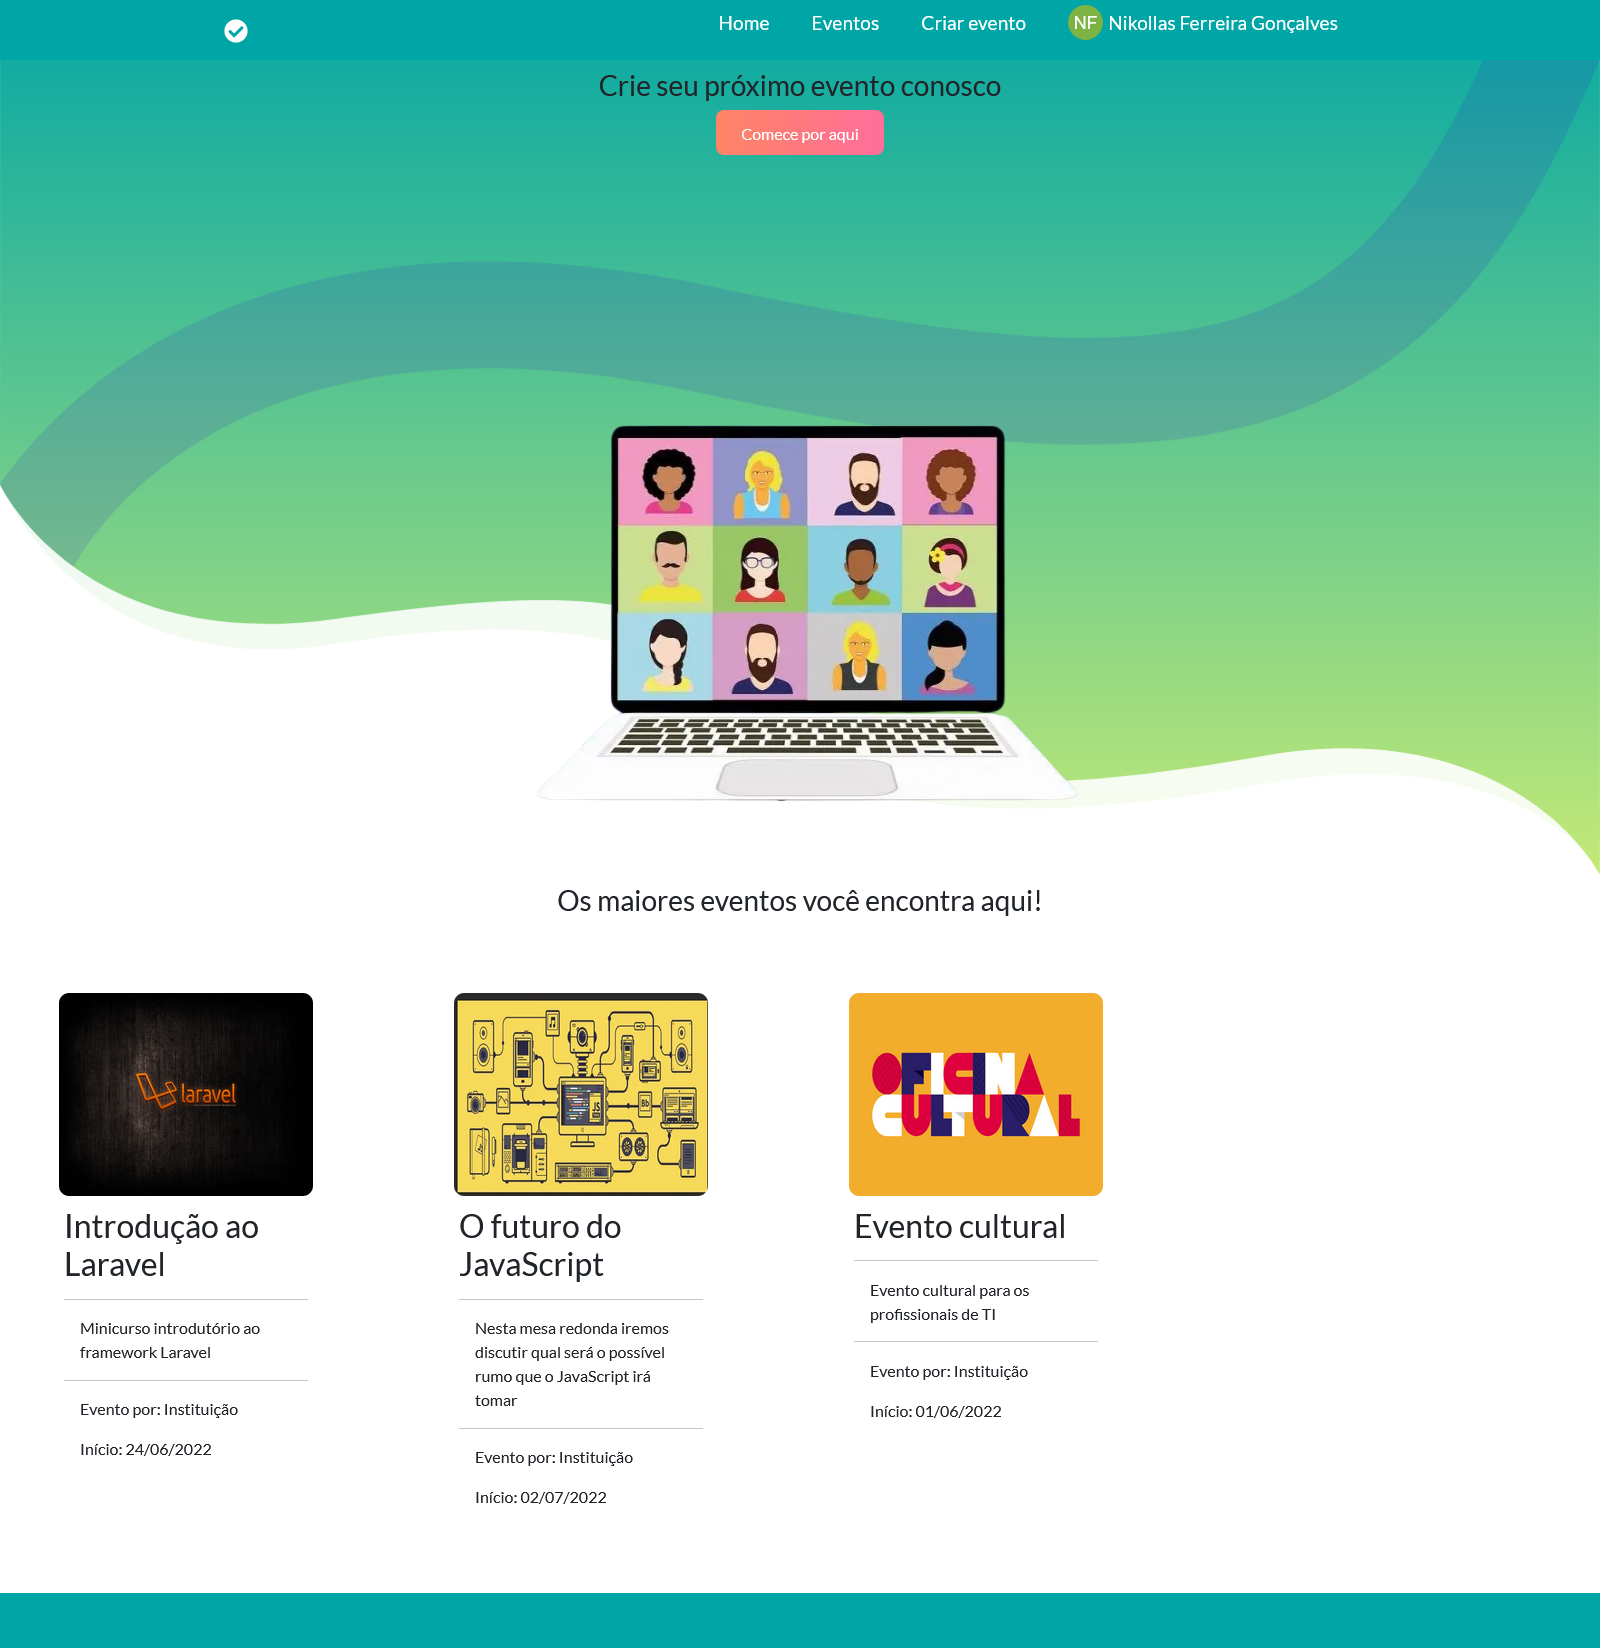
\includegraphics[scale=.23]{home.png}
    \vspace{5pt}
    \legend{Fonte: Próprio autor}
\end{figure}
\begin{figure}[H]
    \caption{\label{login}Página de login}
    \vspace{5pt}
    \centering
    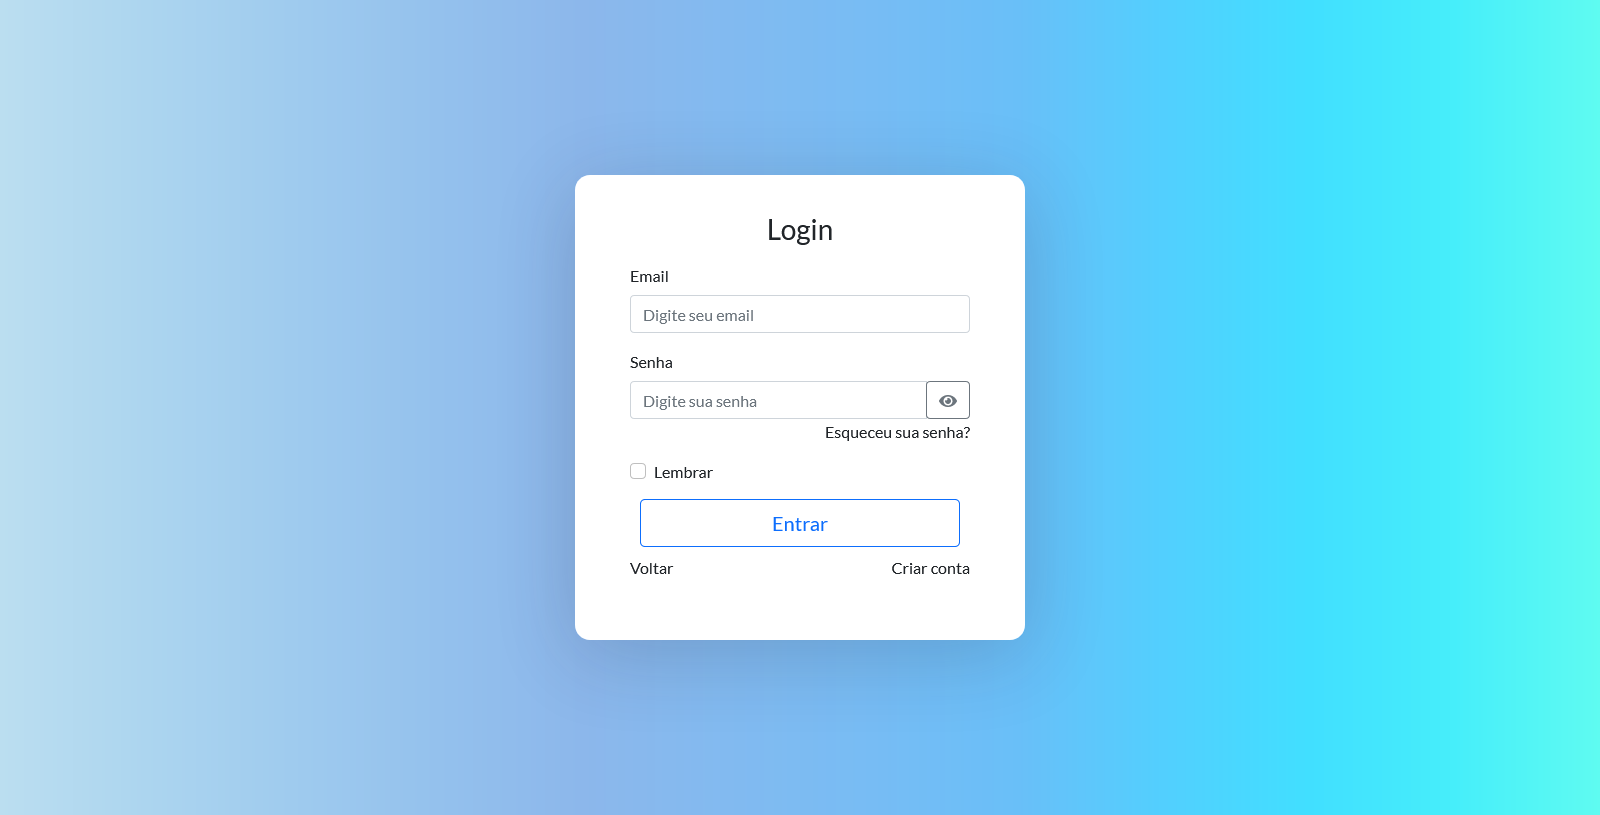
\includegraphics[scale=.25]{login.png}
    \vspace{5pt}
    \legend{Fonte: Próprio autor}
\end{figure}

Utilizando a página inicial como exemplo, é possível ver a responsividade adaptada a ela por meio das figuras \ref{homemob1} e \ref{homemob2}, que se adaptam a um smartphone. A diferença entre o tamanho de tela de um desktop para um smartphone fez com que a \textit{navbar} seja oculta e as imagens dos eventos sejam exibidas apenas uma por linha, dimensionando a imagem para isto.

\begin{figure}[H]
    \caption{\label{homemob1}Página inicial \textit{mobile}}
    \vspace{5pt}
    \centering
    
\includegraphics[scale=.15]{homemob1.jpg}
    \vspace{5pt}
    \legend{Fonte: Próprio autor}
\end{figure}

\begin{figure}[H]
    \caption{\label{homemob2}Continuação da página inicial \textit{mobile}}
    \vspace{5pt}
    \centering
    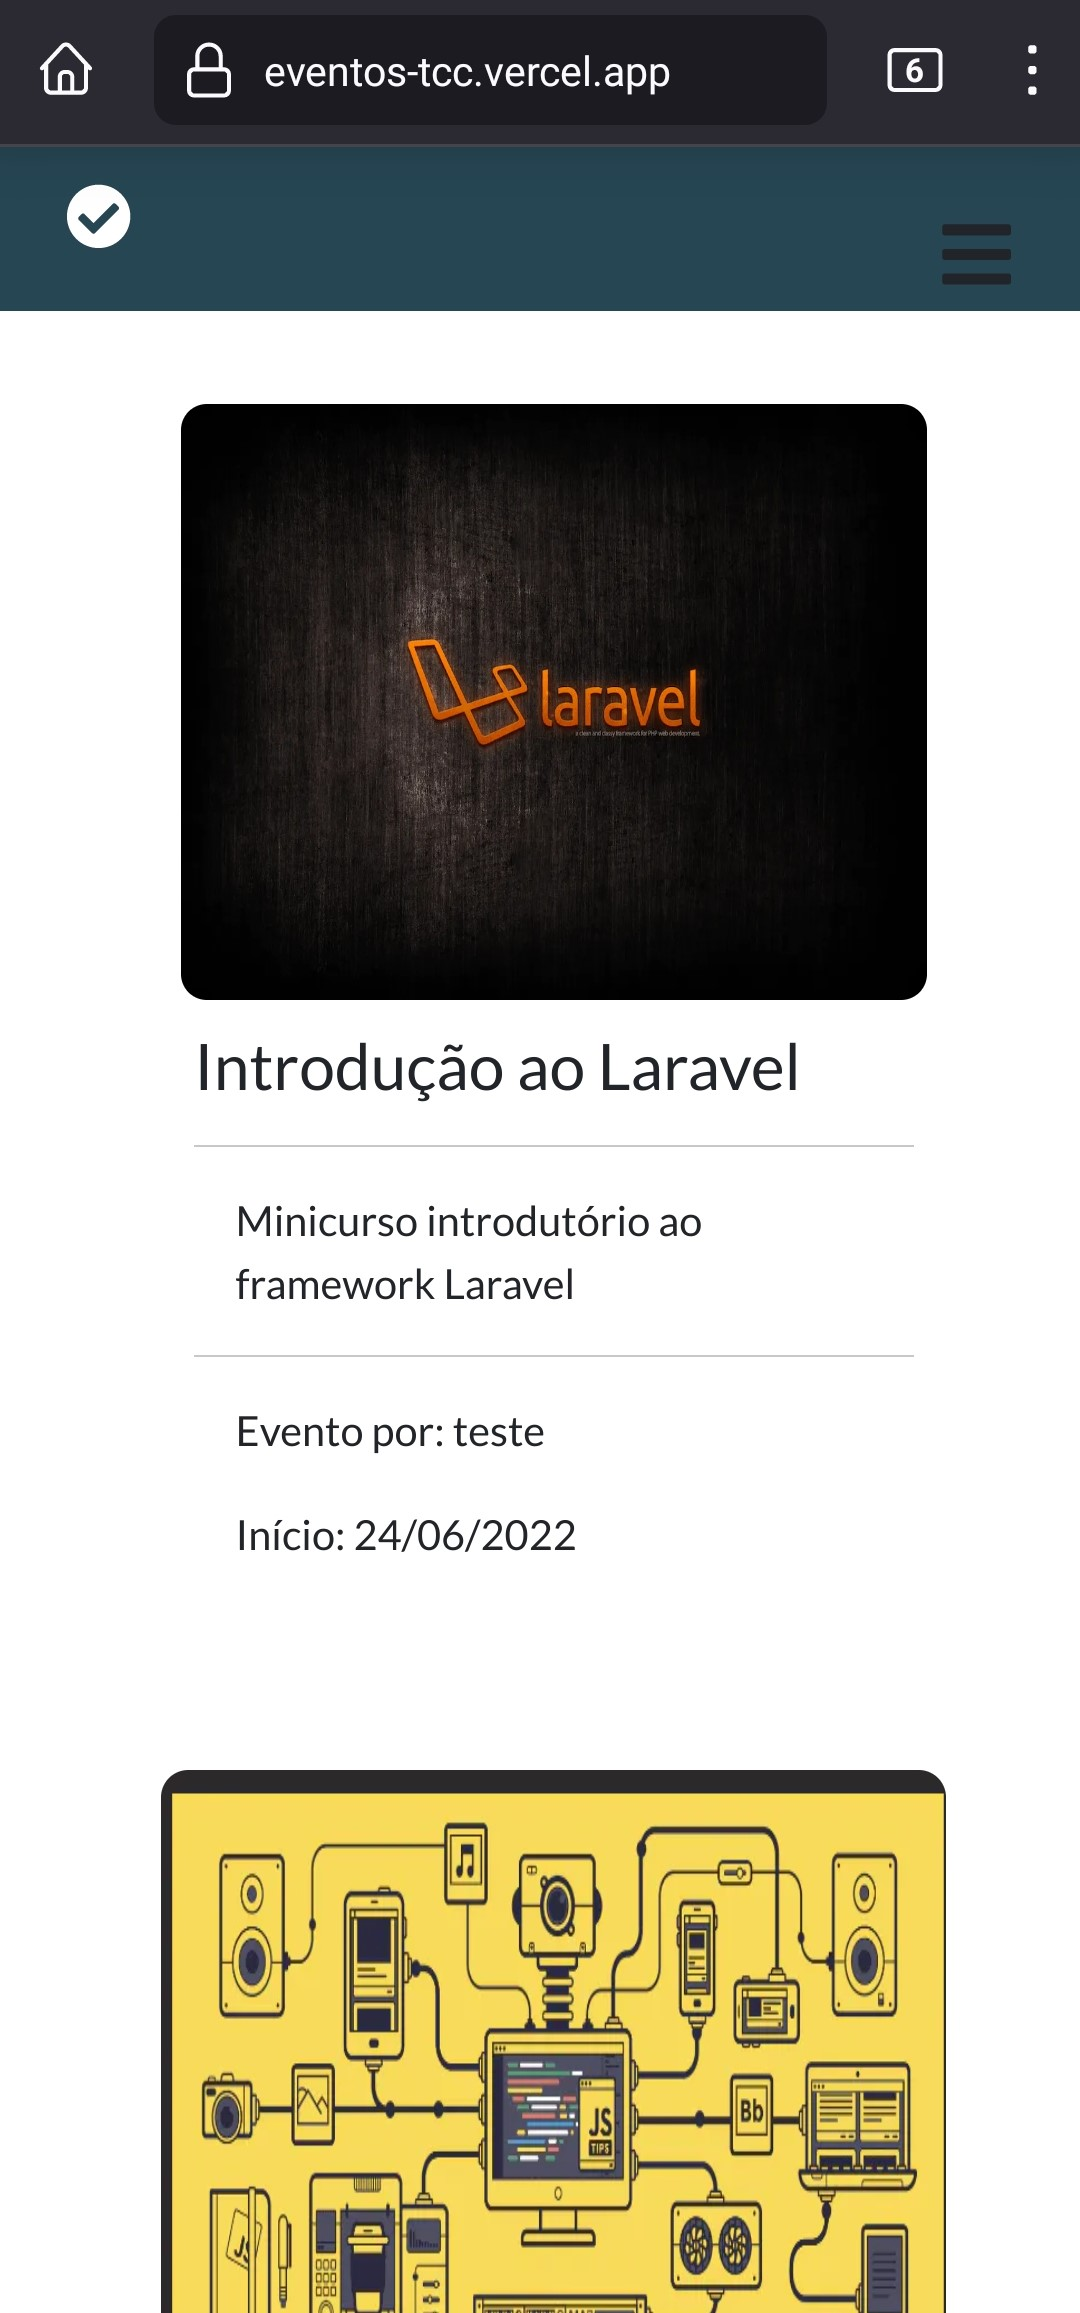
\includegraphics[scale=.15]{homemob2.jpg}
    \vspace{5pt}
    \legend{Fonte: Próprio autor}
\end{figure}

A fluidez, conforme as estatísticas capturadas pela Vercel, foi obtida por meio de carregamento rápido das páginas juntamente com a otimização de imagens fornecidas pelo framework Next.js. A imagem \ref{estVercel} demonstram os dados capturados e suas estatísticas disponíveis no plano gratuito, com o maior problema sendo a primeira impressão dos dados na tela(\textit{First Contentful Paint}), que demonstra o primeiro carregamento dos dados no cliente. Este resultado é esperado, devido ao cache do framework, armazenado em seu servidor após o primeiro uso, o que decai ao longo do tempo, devido a este fator.

\begin{figure}[H]
    \caption{\label{estVercel}Estatísticas Vercel \textit{mobile}}
    \vspace{5pt}
    \centering
    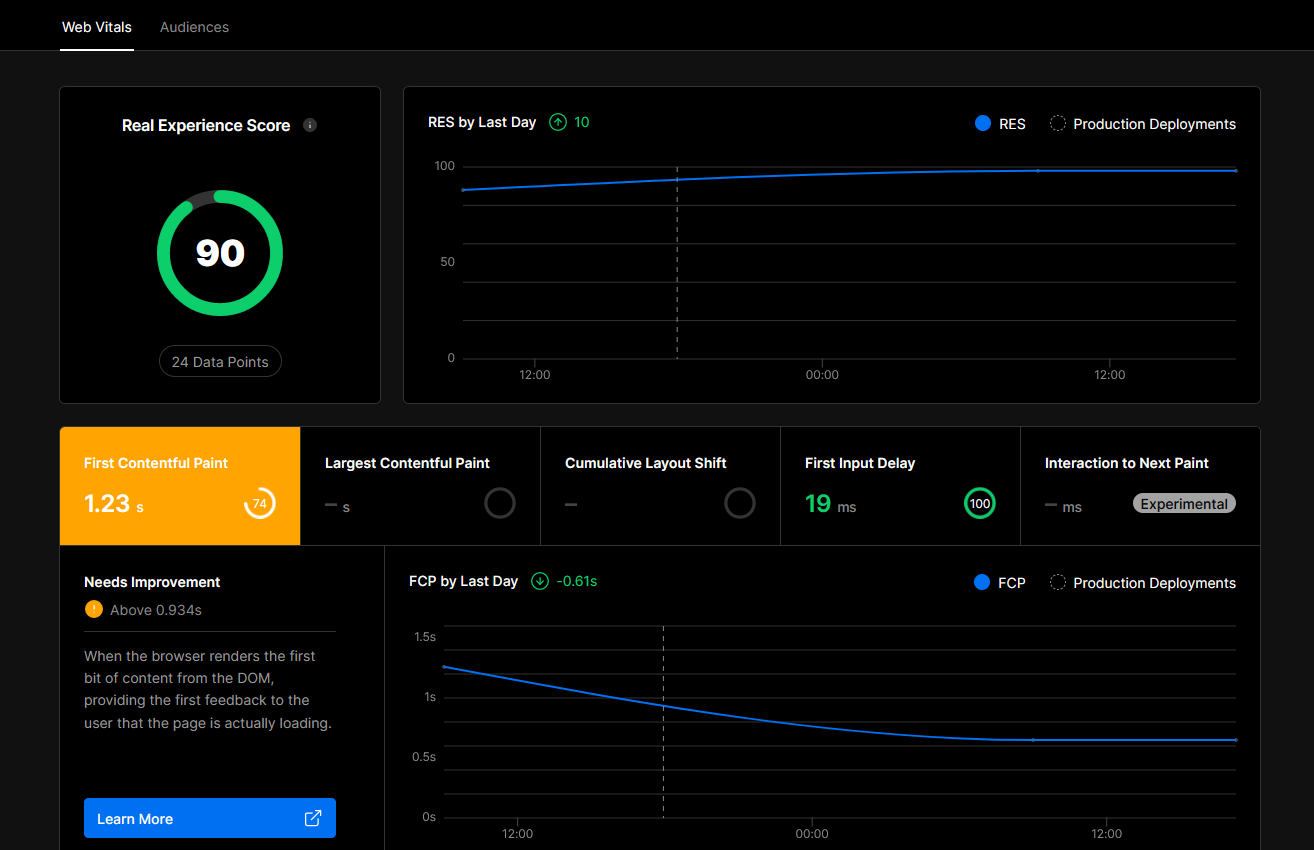
\includegraphics[scale=.3]{vercel_dados.png}
    \vspace{5pt}
    \legend{Fonte: Próprio autor}
\end{figure}

Foi criada uma exibição padrão para cada evento, seguindo o modelo de mockup. Com isto, a aplicação segue um modelo padrão para cada evento, modificando apenas as informações com as imagens contidas em cada um. Na figura \ref{evento}, é possível ver o detalhamento do evento em si e, com a figura \ref{atividades} (que estão na mesma página), tem-se completamente os dados para a participação do usuário, com a descrição completa de quem e o que será apresentado no evento. 

\begin{figure}[H]
    \caption{\label{evento}Página de evento}
    \vspace{5pt}
    \centering
    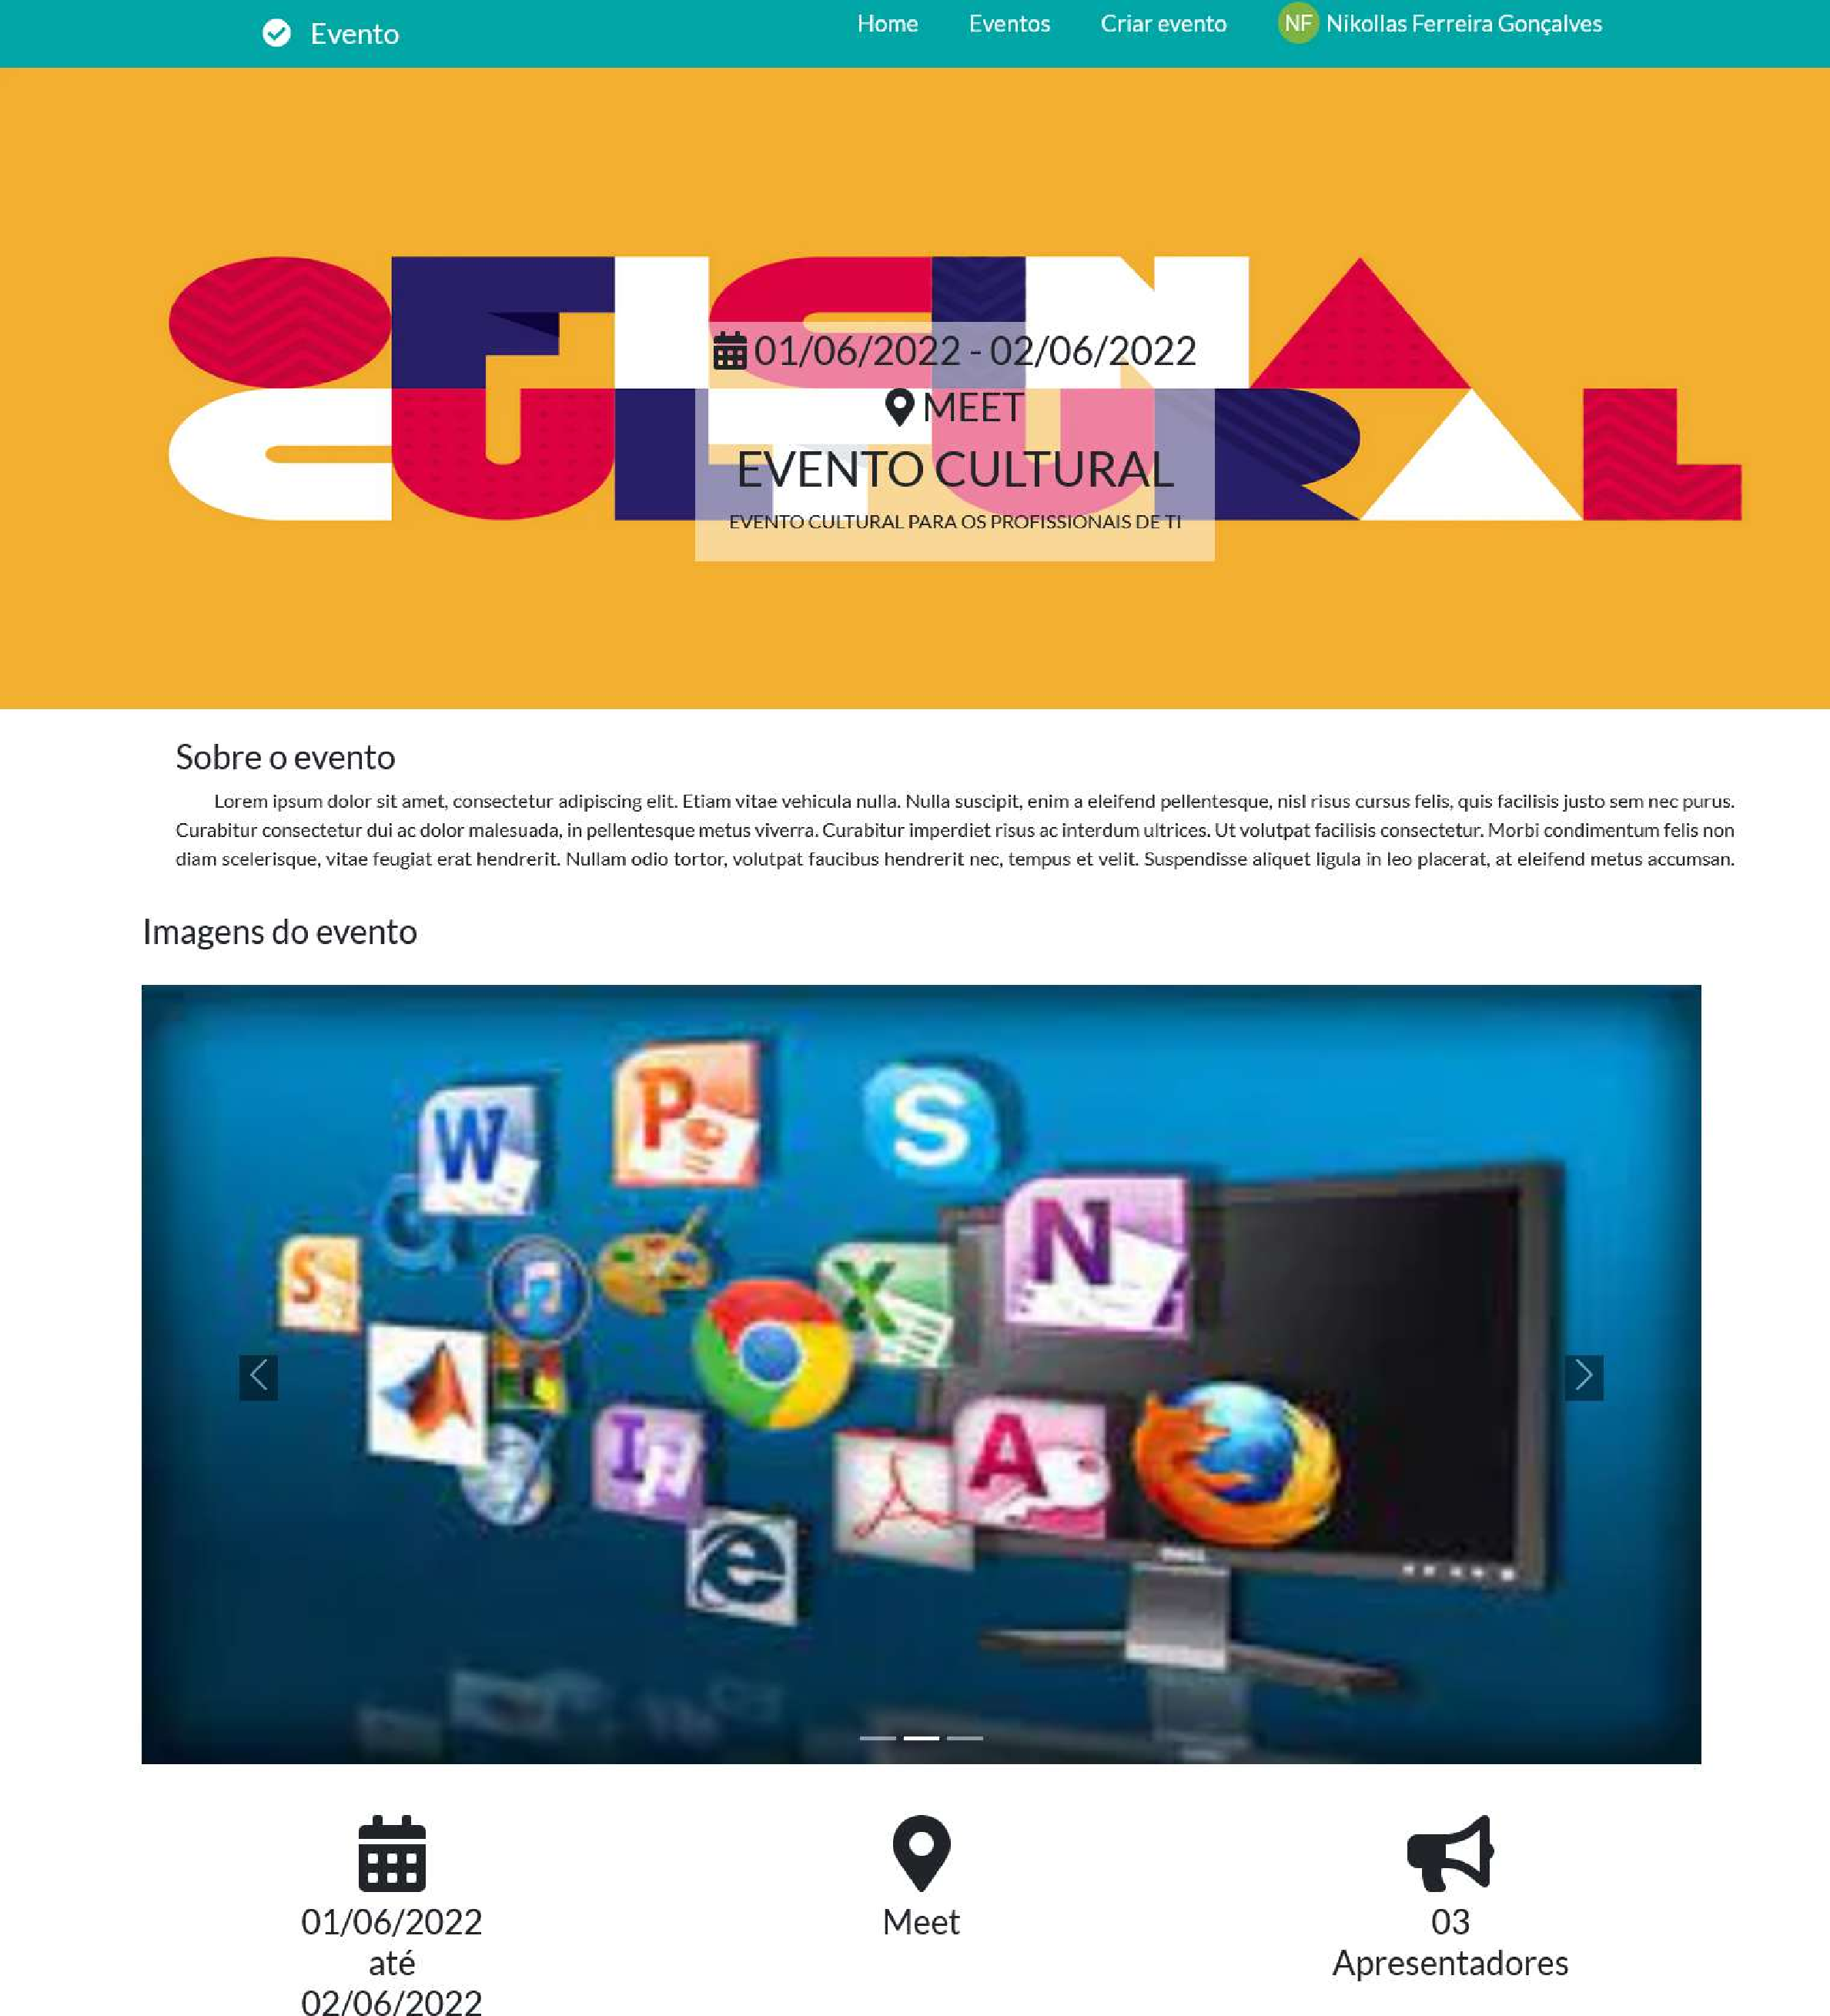
\includegraphics[scale=0.25]{evento.pdf}
    \vspace{5pt}
    \legend{Fonte: Próprio autor}
\end{figure}
\begin{figure}[h]
    \caption{\label{atividades}Atividades}
    \vspace{5pt}
    \centering
    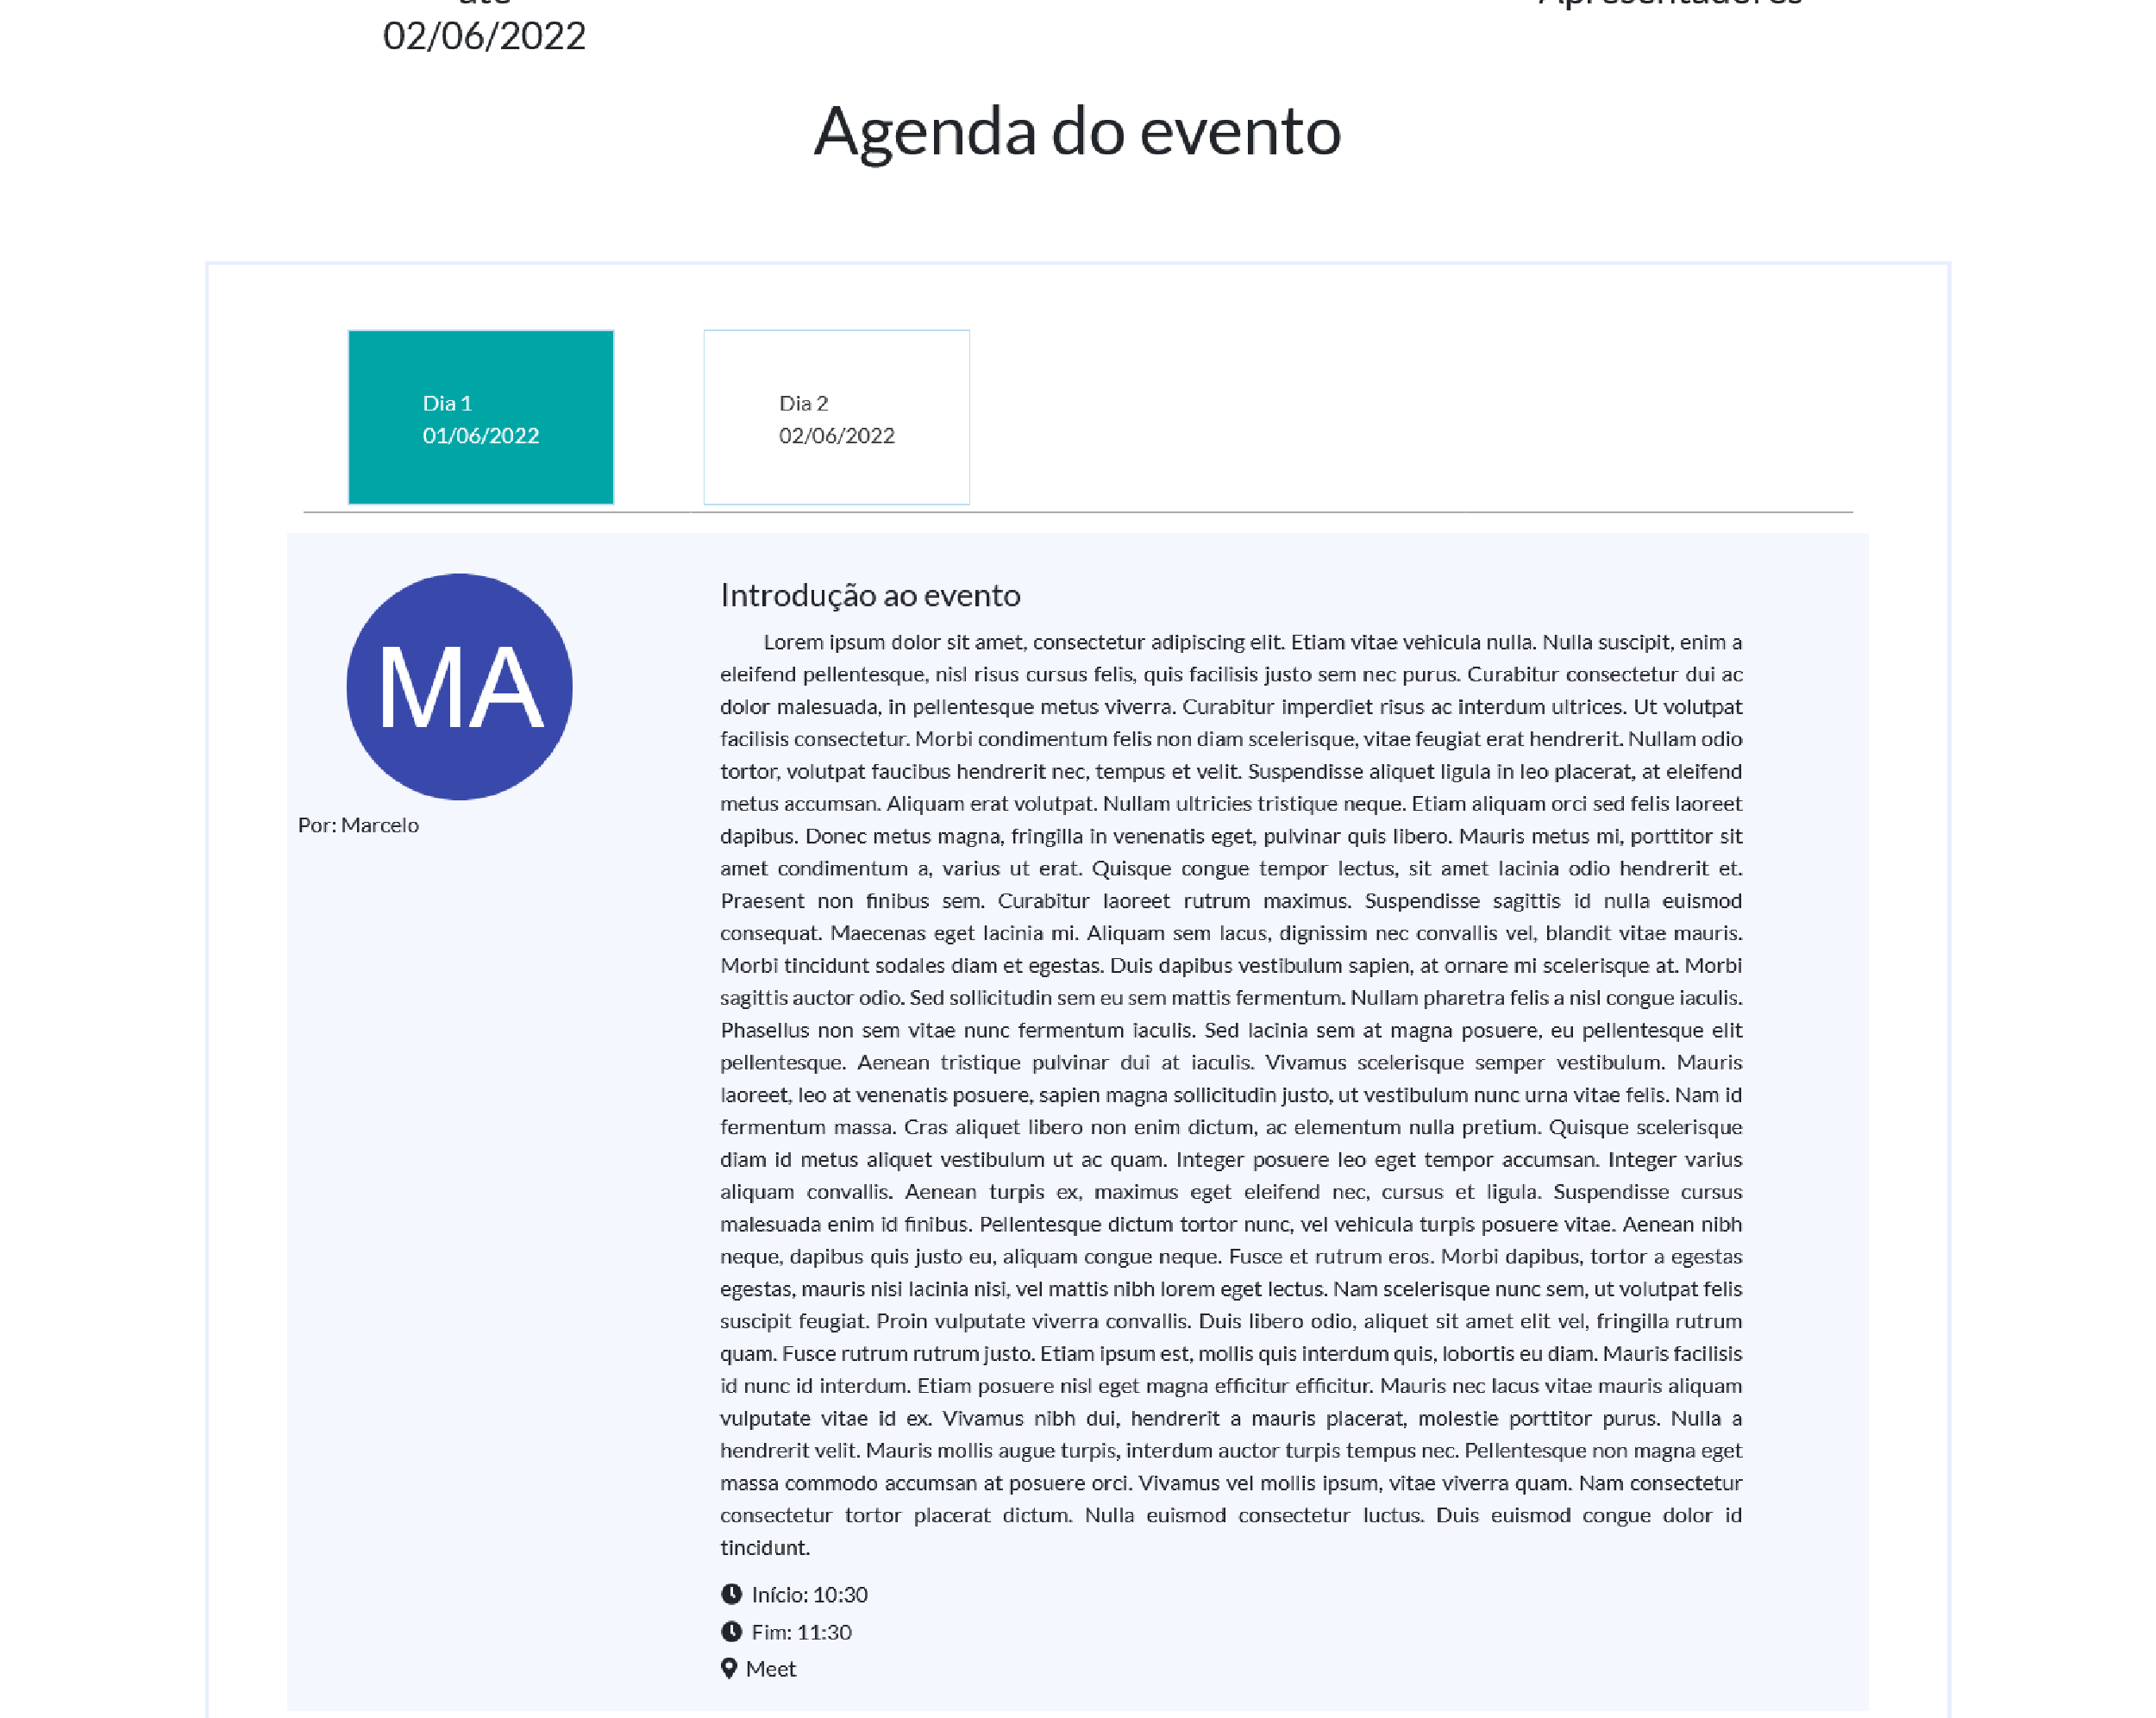
\includegraphics[scale=.25]{atividades.pdf}
    \vspace{5pt}
    \legend{Fonte: Próprio autor}
\end{figure}
%Seguindo para a tela de usuário, a qual será utilizada para gerenciamento de certificados, assim como de eventos, conforme previsto no mockup inicial, apenas alguns detalhes foram ajustados, como ajustes em alguns efeitos visuais de componentes da tela. Então, o que se altera são a quantidade de opções para cada uma das funções descritas anteriormente, como mostram a figura 21, figura 22 e a figura 23, sendo a primeira de um usuário comum, a segunda de um associado e a última de um administrador.\\
O modelo de certificado criado e que pode ser enviado em formato de PDF para o e-mail do participante, incluindo neste caso o apresentador também, também é gerido pela aplicação. Então, foi necessário criar um validador e enviar juntamente ao PDF o código para validação, como demonstrado na figura \ref{certificado}.

\begin{figure}[H]
    \caption{\label{certificado}Exemplo de certificado}
    \vspace{5pt}
    \centering
    
\includegraphics[scale=.20, angle=-90]{certificado-1.jpg}
    \vspace{5pt}
    \legend{Fonte: Próprio autor}
\end{figure}

A criação do \textit{backend} que foi realizada apresenta um token JWT para autenticação e validação dos dados do usuário, além de realizar toda a troca de informações por meio de sua API REST e envio de e-mails dos certificados. Neste, é proporcionado um ambiente e troca de informações seguros por meio das requisições feitas pelo Next.js. Além disso, toda a estruturação inicial planejada foi seguida, com exceções de tabelas auxiliares criadas pelo próprio framework Laravel para facilitar gravações de suas estatísticas e informações essenciais ele, ou seja, toda a cardinalidade das tabelas, assim como o projeto das requisições foi seguido conforme planejado anteriormente.

Por se tratar de um framework bem estruturado e organizado, com o Laravel, foi possível criar um padrão para o projeto que apresente funções bem determinadas e cumprindo o requisito de estarem em seu local, como os Controllers tendo as funções de comunicação com o banco de dados, assim como o retorno da requisição por meio de uma resposta em JSON, e as rotas chamando cada uma dessas funções para serem executadas. Portanto, isto facilitou o desenvolvimento, criando-se um padrão pré-determinado e podendo ser expandido ainda mais para projetos em maiores escalas.

O protótipo da aplicação apresenta uma estrutura bem subdividida, contendo o \textit{frontend} e o \textit{backend} estruturados pelos seus frameworks, podendo ser escalável.

A geração dinâmica dos certificados é uma característica relevante da aplicação que padroniza em uma instituição como podem ser seus documentos. Os modelos podem ser replicados ou diferentes para cada evento, podendo tornar padrão ou exclusivo para cada uso. A API permite a possibilidade de a criação de um aplicativo para \textit{smartphones} sem a necessidade de refazer ou reestruturar o \textit{backend}, devido à implementação de tecnologias como o JSON e ser acessível via protocolo HTTP. Os dados na API são protegidos por meio da autenticação fornecida pelo Laravel, ou seja, os dados da aplicação só serão repassados para quem estiver autenticado e com permissão de acesso a determinadas informações por meio do JWT daquele usuário, que tem prazo de validade. 

Para trabalhos futuros, é necessário que tenha integração com APIs de \textit{gateway} de pagamentos para fornecer à aplicação funcionalidades de ingressos pagos, seja via cartão de crédito/débito ou pix, visto que nem sempre um evento pode ser algo gratuito. A aplicação poderá fazer uma reserva mediante a confirmação do pagamento, gerando um identificador único ao ingresso e podendo ser apresentado em formato de \textit{qrcode} ou o texto do código em si, que deve ser validado ao comparecer às atividades compradas. 

Neste capítulo, foram apresentados os resultados do protótipo desenvolvido. A aplicação é capaz do gerenciamento de eventos, criação e edição dos usuários, assim como geração e validação dos certificados. Pode-se agregar diversas outras funcionalidades a este projeto, dado os frameworks e linguagens utilizados, sendo um protótipo que pode ser viabilizado e implementado em diversas instituições para seu uso no gerenciamento destas tarefas. As funcionalidades estão disponíveis na seguinte URL: \url{https://eventos-tcc.vercel.app/}, o repositório contendo o \textit{frontend} está disponível em \url{https://github.com/NikFG/evento_front} e o repositório do \textit{backend} está disponível em: \url{https://github.com/NikFG/eventos_api}.
